% fig1.tex -- the mechanism, as a TikZ draft (no numbers). Compiles on its own:
%   pdflatex fig1.tex      -> fig1.pdf, then \includegraphics{figs/fig1}
% Colors are the figure palette's blue and orange (paper/figs/style.py).
% Left: a small graph (start, one path to the target, an off-path branch, the
% decoy in its own component). Right: the prompt as tokens, the four latent
% positions, the thought each one emits (reached set growing; the last two
% hold the winner), and the three readers.
\documentclass[tikz,border=3pt]{standalone}
\usetikzlibrary{arrows.meta,calc}
\definecolor{pblue}{HTML}{2A78D6}
\definecolor{porange}{HTML}{EB6834}
\definecolor{pgrey}{HTML}{8A8986}
\begin{document}
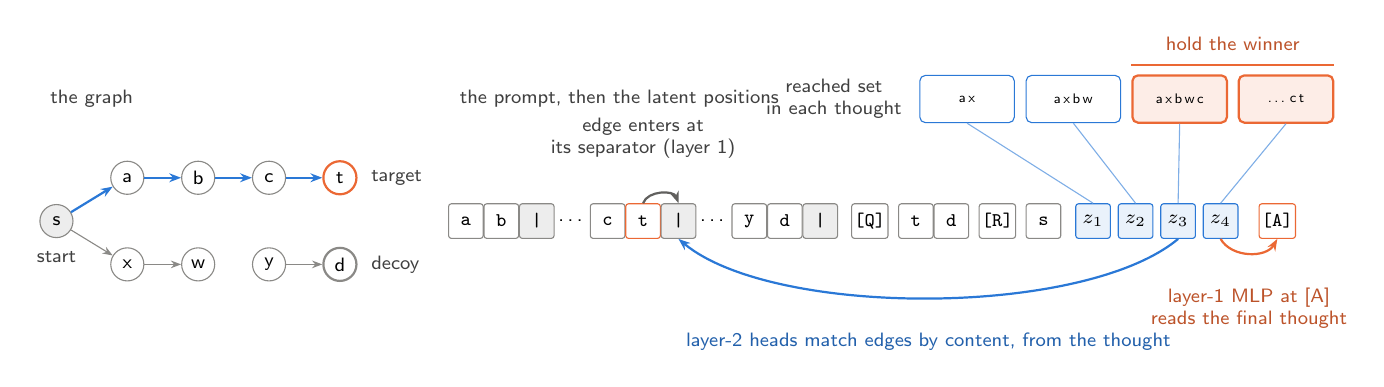
\begin{tikzpicture}[
  font=\sffamily\scriptsize,
  tok/.style={draw=pgrey, rounded corners=1pt, minimum height=4.4mm, minimum width=4.4mm,
              inner sep=1pt, font=\ttfamily\scriptsize},
  sep/.style={tok, fill=pgrey!15},
  lat/.style={tok, draw=pblue, fill=pblue!10, font=\sffamily\scriptsize},
  gnode/.style={circle, draw=pgrey, inner sep=0pt, minimum size=4.2mm},
  gedge/.style={-{Stealth[length=1.3mm]}, pgrey},
  gpath/.style={-{Stealth[length=1.5mm]}, thick, pblue},
  thought/.style={draw=pblue, rounded corners=2pt, minimum width=12mm, minimum height=6mm,
                  align=center, inner sep=1.5pt, font=\sffamily\tiny},
  winner/.style={thought, thick, draw=porange, fill=porange!12},
  call/.style={-{Stealth[length=1.5mm]}, thick},
  note/.style={font=\sffamily\scriptsize, text=black!75, align=center},
]

% ---------------- the graph ----------------
\node[gnode, fill=pgrey!15] (s) at (0, 0)    {s};
\node[gnode] (a) at (0.9, 0.55)  {a};
\node[gnode] (x) at (0.9, -0.55) {x};
\node[gnode] (b) at (1.8, 0.55)  {b};
\node[gnode] (w) at (1.8, -0.55) {w};
\node[gnode] (c) at (2.7, 0.55)  {c};
\node[gnode, draw=porange, thick] (t) at (3.6, 0.55) {t};
\node[gnode] (y) at (2.7, -0.55) {y};
\node[gnode, thick] (d) at (3.6, -0.55) {d};
\draw[gpath] (s) -- (a);
\draw[gpath] (a) -- (b);
\draw[gpath] (b) -- (c);
\draw[gpath] (c) -- (t);
\draw[gedge] (s) -- (x);
\draw[gedge] (x) -- (w);
\draw[gedge] (y) -- (d);
\node[note, below=0.5mm] at (s.south) {start};
\node[note, right=0.5mm] at (t.east) {target};
\node[note, right=0.5mm] at (d.east) {decoy};
\node[note, anchor=west] at (-0.2, 1.55) {the graph};

% ---------------- the prompt ----------------
\def\dx{0.45}
\node[tok] (e1s) at (5.2, 0) {a};
\node[tok] (e1t) at ($(e1s)+(\dx,0)$) {b};
\node[sep] (e1p) at ($(e1t)+(\dx,0)$) {|};
\node at ($(e1p)+(\dx,0)$) {\dots};
\node[tok] (e2s) at ($(e1p)+(2*\dx,0)$) {c};
\node[tok, draw=porange] (e2t) at ($(e2s)+(\dx,0)$) {t};
\node[sep] (e2p) at ($(e2t)+(\dx,0)$) {|};
\node at ($(e2p)+(\dx,0)$) {\dots};
\node[tok] (e3s) at ($(e2p)+(2*\dx,0)$) {y};
\node[tok] (e3t) at ($(e3s)+(\dx,0)$) {d};
\node[sep] (e3p) at ($(e3t)+(\dx,0)$) {|};
\node[tok] (q)  at ($(e3p)+(1.4*\dx,0)$) {[Q]};
\node[tok] (c1) at ($(q)+(1.3*\dx,0)$) {t};
\node[tok] (c2) at ($(c1)+(\dx,0)$) {d};
\node[tok] (r)  at ($(c2)+(1.3*\dx,0)$) {[R]};
\node[tok] (rt) at ($(r)+(1.3*\dx,0)$) {s};
\node[lat] (z1) at ($(rt)+(1.4*\dx,0)$) {$z_1$};
\node[lat] (z2) at ($(z1)+(1.2*\dx,0)$) {$z_2$};
\node[lat] (z3) at ($(z2)+(1.2*\dx,0)$) {$z_3$};
\node[lat] (z4) at ($(z3)+(1.2*\dx,0)$) {$z_4$};
\node[tok, draw=porange] (ans) at ($(z4)+(1.6*\dx,0)$) {[A]};
\node[note, anchor=west] at (5.0, 1.55) {the prompt, then the latent positions};

% ---------------- the thoughts: the reached set grows ----------------
\node[thought] (th1) at ($(z1)+(-1.6,1.55)$) {a\,x};
\node[thought] (th2) at ($(th1)+(1.35,0)$) {a\,x\,b\,w};
\node[winner]  (th3) at ($(th2)+(1.35,0)$) {a\,x\,b\,w\,c};
\node[winner]  (th4) at ($(th3)+(1.35,0)$) {\dots\,c\,t};
\foreach \i in {1,...,4} \draw[pblue!60] (z\i.north) -- (th\i.south);
\node[note, anchor=east] at ($(th1.west)+(-0.1,0)$) {reached set\\in each thought};
\draw[porange, thick] ($(th3.north west)+(0,0.12)$) -- ($(th4.north east)+(0,0.12)$);
\node[note, text=porange!80!black, above=0.6mm] at ($(th3.north)!0.5!(th4.north)+(0,0.12)$) {hold the winner};

% ---------------- the three readers ----------------
% 1. an edge enters at its separator: layer 1 copies the slot into "|"
\draw[call, pgrey!70!black] (e2t.north) to[bend left=70] (e2p.north);
\node[note, above=4.5mm] at (e2t.north) {edge enters at\\its separator (layer 1)};
% 2. layer-2 heads match edges by content, from the thought's query
\draw[call, pblue] (z3.south) .. controls ($(z3.south)+(-1.2,-1.0)$) and ($(e2p.south)+(1.2,-1.0)$) .. (e2p.south);
\node[note, text=pblue!80!black] at ($(e2p.south)!0.5!(z3.south)+(0,-1.3)$) {layer-2 heads match edges by content, from the thought};
% 3. the answer position's layer-1 MLP reads the final thought
\draw[call, porange] (z4.south) to[bend right=60] (ans.south);
\node[note, text=porange!80!black, below=5mm] at ($(z4.south)!0.5!(ans.south)$) {layer-1 MLP at [A]\\reads the final thought};

\end{tikzpicture}
\end{document}
